\documentclass{beamer}

\usepackage[english]{babel}
\usepackage{multirow}
\usepackage{amsmath,amsthm}
\usepackage{amsfonts}
\usepackage{xkeyval}
\usepackage{graphics}
\usepackage{url}
\usepackage[lined,boxed,linesnumbered]{algorithm2e}
\usepackage{CJKutf8} %支持中文

\mode<presentation>
{
  %\usetheme{}
  %\usecolortheme{beaver}
  % 可供选择的主题参见 beameruserguide.pdf, 第 134 页起
  % 无导航条的主题: Bergen, Boadilla, Madrid, Pittsburgh, Rochester;
  % 有树形导航条的主题: Antibes, JuanLesPins, Montpellier;
  % 有目录竖条的主题: Berkeley, PaloAlto, Goettingen, Marburg, Hannover;
  % 有圆点导航条的主题: Berlin, Dresden, Darmstadt, Frankfurt, Singapore, Szeged;
  % 有节与小节导航条的主题: Copenhagen, Luebeck, Malmos, Warsaw
  %\setbeamercovered{transparent}
  % 如果取消上一行的注解 %, 就会使得被覆盖部分变得透明(依稀可见)
}
\definecolor{kugreen}{RGB}{160,63,171}
\definecolor{kugreenlys}{RGB}{132,158,139}
\definecolor{kugreenlyslys}{RGB}{173,190,177}
\definecolor{kugreenlyslyslys}{RGB}{214,223,216}
\setbeamercovered{transparent} %设置半透明化尚未出现的内容
\mode<presentation>
{
  \usetheme{PaloAlto}
  \usecolortheme[named=kugreen]{structure}
  \useinnertheme{circles}
  \usefonttheme[onlymath]{serif}
  \setbeamercovered{transparent}
  \setbeamertemplate{blocks}[rounded][shadow=true]
}

\newcommand{\myblock}[1]{\begin{block}{}#1\end{block}}

\logo{
\includegraphics[scale=0.08]{images/HUSTLogo}}%Logo of the presentation
\title{Training RBM}
\author{Yunfei Wang}
\institute{Department of Computer Science \& Technology \\ Huazhong University of Science \& Technology}
\date{\today}

\begin{document}

\begin{CJK*}{UTF8}{gbsn} %中文支持

\begin{frame}
\titlepage
\end{frame}


\begin{frame}\frametitle{Table of contents}
\tableofcontents
\end{frame}

\section{Restricted Boltzmann Machine(RBM)}
\subsection{Relevant Concepts and Basic Properties}
\begin{frame}[allowframebreaks]\frametitle{RBM}
\begin{columns} % the "c" option specifies top vertically alignment
\begin{column}{0.5\textwidth}% column designated by a command
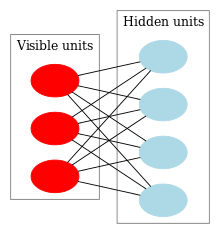
\includegraphics[scale=0.5]{images/RBM}
\end{column}
\begin{column}{0.5\textwidth}
\myblock{Undirected bipartite graph}
\myblock{Visible units $v\in\{0,1\}^D$ Feature of inputs}
\myblock{Hidden units $h\in\{0,1\}^F$ Feature detectors}
\end{column}
\end{columns}
The energy of joint distribution:
\begin{equation}
E(v,h;\theta)=-v^TWh-a^Tv-b^Th
\end{equation}
$\theta={W,a,b}$ are the model parameters.

The probability of each pair of a visible and a hidden vector:
\begin{equation}
P(v,h;\theta)=\frac{1}{Z(\theta)}\exp(-E(v,h;\theta))
\end{equation}
Partition function(Normalizing Constant):
\begin{equation}
Z(\theta)=\sum_{v,h}\exp(-E(v,h;\theta))
\end{equation}

Marginal distribution:
\begin{equation}
\begin{split}
P(v;\theta)&=\sum_hP(v,h;\theta)\\
&=\frac{1}{Z(\theta)}\sum_h \exp(v^TWh+a^Tv+b^Th)\\
&=\frac{1}{Z(\theta)}\exp(a^Tv)\sum_h \exp(v^TWh+b^Th)\\
&=\frac{1}{Z(\theta)}\exp(a^Tv)\prod_{j=1}^F\sum_{h_j\in\{0,1\}}\exp(\sum_{i=1}^Dv_iW_{ij}h_j+b_jh_j)\\
&=\frac{1}{Z(\theta)}\exp(a^Tv)\prod_{j=1}^F(1+\exp(\sum_{i=1}^Dv_iW_{ij}+b_j))
\end{split}
\end{equation}

Conditional distribution over visible units can be figured out using Bayesian formula:
\begin{equation}
\begin{split}
P(h|v;\theta)&=\frac{P(v,h;\theta)}{P(v;\theta)}\\
&=\frac{\exp(v^TWh+b^Th)}{\prod_{j=1}^F(1+\exp(\sum_{i=1}^Dv_iW_{ij}+b_j))}\\
&=\prod_{j=1}^F\frac{\exp(\sum_{i=1}^Dv_iW_{ij}h_j+b_jh_j)}{1+\exp(\sum_{i=1}^Dv_iW_{ij}+b_j)}
\end{split}
\end{equation}

The hidden units are conditionally independent:
\begin{equation}
P(h|v;\theta)=\prod_{j=1}^FP(h_j|v;\theta)=\prod_{j=1}^F\frac{exp(\sum_{i=1}^Dv_iW_{ij}h_j+b_jh_j)}{1+exp(\sum_{i=1}^Dv_iW_{ij}+b_j)}
\end{equation}

It's easy to derive the following conclusions:
\begin{equation}
P(h_j|v)=\frac{\exp(\sum_{i=1}^Dv_iW_{ij}h_j+b_jh_j)}{1+\exp(\sum_{i=1}^Dv_iW_{ij}+b_j)}
\end{equation}
\begin{equation}
\begin{split}
P(h_j=1|v)&=\frac{\exp(\sum_{i=1}^Dv_iW_{ij}+b_j)}{1+\exp(\sum_{i=1}^Dv_iW_{ij}+b_j)}\\
&=\frac{1}{1+\exp(-\sum_{i=1}^Dv_iW_{ij}-b_j)}\\
&=g(\sum_{i=1}^Dv_iW_{ij}+b_j)
\end{split}
\end{equation}
where $g(x)=\frac{1}{1+\exp(-x)}$ is the logistic function.

Similarly:
\begin{equation}
P(v|h;\theta)=\prod_{i=1}^FP(v_i|h;\theta)
\end{equation}
\begin{equation}
P(v_i=1|h)=g(\sum_{j=1}^FW_{ij}h_j+a_i)
\end{equation}

\begin{figure}
  % Requires \usepackage{graphicx}
  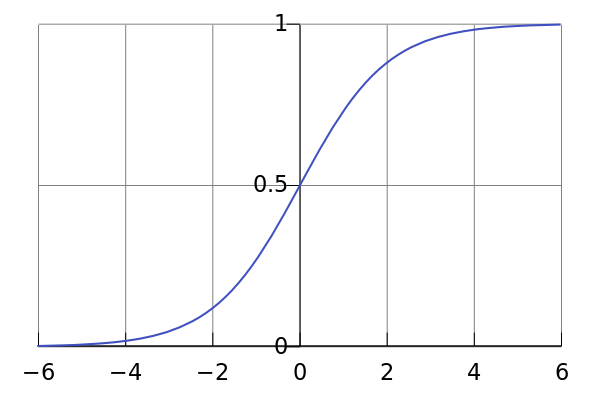
\includegraphics[scale=0.18]{images/sigmoidfun}
  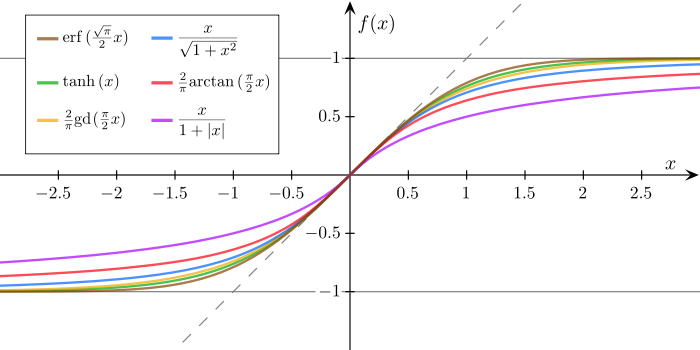
\includegraphics[scale=0.2]{images/sigmoidfun2}\\
  \caption{Sigmoid function:bounded, differentiable, real-valued}
\end{figure}

Log-likelihood:
\begin{equation}
\log P(v;\theta)=\log\sum_h\exp(-E(v,h;\theta))-\log Z
\end{equation}

Derivative of the log-likelihood with respect to parameters $\theta$:
\begin{equation}
\begin{split}
\frac{\partial P(v;\theta)}{\partial W}&=\frac{\sum_hvh^T\exp(-E(v,h;\theta))}{\sum_h\exp(-E(v,h;\theta))}-\frac{\sum_{v,h}vh^T\exp(-E(v,h;\theta))}{Z(\theta)}\\
&=\frac{\sum_hvh^TP(v,h;\theta)}{P(v;\theta)}-\sum_{v,h}vh^TP(v,h;\theta)\\
&=\sum_hvh^TP(h|v;\theta)-\sum_{v,h}vh^TP(v,h;\theta)\\
&=E_{data}(vh^T)-E_{model}(vh^T)
\end{split}
\end{equation}

Similarly:
\begin{equation}
\frac{\partial P(v;\theta)}{\partial a}=E_{data}(v)-E_{model}(v)
\end{equation}
\begin{equation}
\frac{\partial P(v;\theta)}{\partial b}=E_{data}(h)-E_{model}(h)
\end{equation}
where $E_{data}(\bullet)$ and $E_{model}(\bullet)$ denote expectations under the distributions specified by data and model respectively.

According to \emph{Gradient Descent},this leads to a learning rule:
\begin{equation}
\triangle W=\alpha(\underbrace{E_{data}(vh^T)}_{\textcolor{green}{tractable}}-\underbrace{E_{model}(vh^T)}_{\textcolor{red}{intractable}})
\end{equation}
where $\alpha$ is the learning rate.
\end{frame}

\subsection{Learning Algorithms}
\begin{frame}[allowframebreaks]\frametitle{Learning Algorithms}
Approximating the gradient of a different objective function,called \textcolor{red}{"Contractive Divergence"}:
\begin{equation}
\triangle W=\alpha(E_{data}(vh^T)-E_{T}(vh^T))
\end{equation}
where $E_{T}(\bullet)$ denote expectation under the distributions defined by running \textcolor{blue}{Gibbs Sampling} for $T$ full steps,starting from a training example:

\begin{block}{What's Gibbs Sampling?}
Gibbs sampling is applicable when the joint distribution is not known explicitly, but the conditional distribution of each variable is known and is easy to sample from.\\
Gibbs sampling algorithm generates an instance from the distribution of each variable in turn, conditional on the current values of the other variables.
\end{block}

\begin{block}{Implementation of Gibbs Sampling}
Obtain samples of $X=\{x_1,x_2,\cdots,x_n\}$ from a joint distribution $P(x_1,x_2,\cdots,x_n)$.Denote the i-th sample by $X^i=\{x_1^i,x_2^i,\cdots,x_n^i\}$.
\begin{equation}
\begin{split}
&x_1^{i+1}\sim P(x_1|x_2^i,x_3^i,\cdots,x_n^i)\\
&x_2^{i+1}\sim P(x_2|x_1^{i+1},x_3^i,\cdots,x_n^i)\\
&x_3^{i+1}\sim P(x_3|x_1^{i+1},x_2^{i+1},\cdots,x_n^i)\\
&\cdot\\
&\cdot\\
&x_n^{i+1}\sim P(x_n|x_1^{i+1},x_2^{i+1},\cdots,x_{n-1}^{i+1})
\end{split}
\end{equation}
A new sample $X^{i+1}=\{x_1^{i+1},x_2^{i+1},\cdots,x_n^{i+1}\}$ is produced here.
\end{block}

\begin{block}{Gibbs Sampling in RBMs}
\begin{figure}
  \centering
  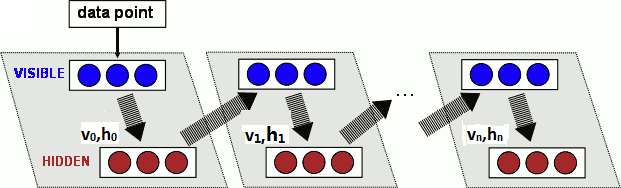
\includegraphics[scale=0.25]{images/GibbsSamp}
  \caption{Gibbs Sampling}
\end{figure}
Start with a training vector on visible units.\\
Update all hidden units in parallel.\\
Update all visible units in parallel to get a "reconstruction".\\
Update the hidden units again.
\end{block}
The change in weight is then given by:
\begin{equation}
\triangle W=\alpha(E_{data}(vh^T)-E_{recon}(vh^T))
\end{equation}
\end{frame}

\subsection{Different types of unit}
\begin{frame}[allowframebreaks]\frametitle{Different types of unit}
\begin{block}{Softmax units}
For a binary unit,the probability of turning on:
\begin{equation}
P(x)=\frac{1}{1+\exp(-x)}=\frac{\exp(x)}{\exp(x)+\exp(0)}\propto\exp(x)
\end{equation}
\textcolor{blue}{Generalize the binary states to $K$ alternative states:}
\begin{equation}
P(x_i)=\frac{\exp(x_i)}{\sum_{k=1}^K\exp(x_k)}
\end{equation}
\textcolor{red}{Softmax unit}:States are mutually constrained;Only one unit has value 1,the rest have value 0;View it as a set of $K$ binary units.\\
\end{block}

\begin{block}{Multinomial units}
\textcolor{cyan}{Useful for modelling sparse count data,such as word count vectors in a document.}Visible units $v\in \mathbb{N}^D$,hidden units $h\in\{0,1\}^F$.The energy function is defined as follows:
\begin{equation}
E(v,h;\theta)=-\sum_{i=1}^D\sum_{j=1}^Fv_iW_{ij}h_j-\sum_{i=1}^Da_iv_i-M\sum_{j=1}^Fb_jh_j
\end{equation}
where $v_i$ is the frequency of word $i$ in a document,$D$ is vocabulary size,$M=\sum_{i=1}^Dv_i$ is total number of words in the document.
This leads to the following conditional distribution:
\begin{equation}
P(v_i=1|h;\theta)=\frac{\exp(-a_i+\sum_{j=1}^FW_{ij}h_j)}{\sum_{i=1}^D\exp(-a_i+\sum_{j=1}^FW_{ij}h_j)}
\end{equation}
%\textcolor{red}{Multinomial unit}:Sampling $N$ times;$K$ different states can have integer values bigger than 1,but values must add to $N$.
\end{block}

\begin{block}{Gaussian visible units}
Solution to a representation for images or speech using logistic units: \textcolor{blue}{replace binary visible units by linear units with independent Gaussian noise}.Visible units $v\in \mathbb{R}^D$,hidden units $h\in\{0,1\}^F$.The energy function is defined as follows:
\begin{equation}
E(v,h;\theta)=\sum_{i=1}^D\frac{(v_i-a_i)^2}{2\sigma_i^2}-\sum_{j=1}^Fb_jh_j-\sum_{i,j}\frac{v_i}{\sigma_i}h_jW_{ij}
\end{equation}
where $\theta=\{a,b,W,\sigma\}$ are the model parameters.
This leads to the following conditional distribution:
\begin{equation}
P(v_i,h;\theta)=\mathcal{N}(a_i+\sigma_i\sum_{j=1}^FW_{ij}h_j,\sigma_i^2)
\end{equation}
\end{block}

\begin{block}{Gaussian visible and hidden units}
Both the visible and hidden units are Gaussian,then the energy function becomes:
\begin{equation}
E(v,h)=\sum_{i\in vis}\frac{(v_i-a_i)^2}{2\sigma_i^2}+\sum_{j\in hid}\frac{(h_j-b_j)^2}{2\sigma_j^2}-\sum_{i,j}\frac{v_i}{\sigma_i}\frac{h_j}{\sigma_j}W_{ij}
\end{equation}
With a sufficiently small learning rate, $CD_1$ can learn an undirected version of a factor analysis model using Gaussian units,which is harder than using EM to learn a directed model.
\end{block}

\end{frame}

%\begin{frame}\frametitle{Pseudo-code of the algorithm}
%\begin{algorithm}[H]
%\KwIn{$A \in \mathbb R^{n \times d},Y \in \mathbb R^{d \times N},\rho$;}
%\KwOut{ID(Y);}
%\emph{Set $B=\left[ A^T,\rho I \right],t=0$}\;
%\emph{Initialize $D_t \in \mathbb R^{(n+d) \times (n+d)}$ as an identity matrix}\;
%\Repeat(\tcp*[h]{Iteratively compute U}){Convergence}
%{
%	Calculate $U_{t+1}=D_t^{-1}B^T(BD_t^{-1}B^T)^{-1}Y$\;
%	Calculate the diagonal matrix $D_{t+1}$,where the i-th diagonal element is $\frac{1}{2\|u_{t+1}^t\|_2}$\;
%	$t=t+1$\;
%}
%\For{$j= 1$ \KwTo $N$}
%{
%	Get $r_s(y_j)=\|y-A^T\delta_s(x_j)\|_2,s=1,2,\cdots ,C$\;
%	$ID(y_i)=\mathop{\min}\limits_{s=1,2,\cdots ,C}r_s(y_j)$\;
%}
%\Return $ID(Y)=((ID(y_1),ID(y_2),\cdots ,ID(y_n))$\;	
%\caption{Classification using $\ell_{2,1}$-norm based regression model}
%\end{algorithm}
%\end{frame}
\end{CJK*}
\end{document}
